% !TeX root = ../Report.tex
\section{Proof of Concept Development}

The development of the Proof of Concept (PoC) followed the software architecture presented in Section~\ref{sec:software architecture}. Rather than implementing all the components simultaneously, the development process adopted a bottom-up approach, starting from the core infrastructure responsible for managing and retrieving the knowledge exploited by the multi-agent system.

Throughout the implementation, particular attention was paid to designing a modular and extensible software architecture. The system was developed by defining clear interfaces and abstract base classes, allowing each component to be extended or replaced with minimal impact on the rest of the framework. This design choice promotes maintainability, scalability, and the integration of alternative implementations as the system evolves.

The first component developed was the \textit{Storage Manager}. Since the effectiveness of the decision support system strongly depends on the quality and accessibility of contextual information, this module was designed as the foundation of the entire architecture. Its implementation includes a Retrieval-Augmented Generation (RAG) system developed from scratch, responsible for document ingestion, indexing, semantic retrieval, and knowledge management.

\subsection{Storage Manager \& RAG System}

The Storage Manager represents the foundational component of the proposed multi-agent framework, providing a centralized infrastructure for document ingestion, indexing, storage, and semantic retrieval. Since the system relies on external knowledge to support their process, this module was developed before the remaining components of the architecture.

Rather than implementing a task-specific Retrieval-Augmented Generation (RAG) pipeline, the objective was to design a modular and extensible framework capable of accommodating different implementations of each stage of the retrieval process. For this reason, the entire Storage Manager follows an abstraction-oriented design, where the main functionalities are defined through abstract base classes and later specialized by concrete implementations.

The resulting architecture separates the RAG pipeline into four independent layers:

\begin{itemize}
    \item document chunking;
    \item embedding generation;
    \item memory management and retrieval;
    \item vector storage.
\end{itemize}

Each layer exposes a common interface while hiding its internal implementation details. Consequently, individual components can be replaced without affecting the remaining modules. For example, changing the embedding model or replacing the vector database only requires implementing the corresponding abstract interface, while the higher-level retrieval logic remains unchanged.

This design significantly improves maintainability, facilitates experimentation with different retrieval strategies, and allows the framework to evolve without requiring substantial modifications to the existing codebase.

\subsubsection{Architecture}

Figure~\ref{fig:rag_architecture} illustrates the overall architecture of the implemented Storage Manager.

The document ingestion process starts from the \texttt{Chunker}, responsible for loading heterogeneous documents and dividing them into semantically coherent chunks. The generated chunks are then converted into dense vector representations through the selected embedding model.

The resulting embeddings, together with their metadata, are stored inside the \texttt{Vector Store}, while a parallel lexical index based on \texttt{BM25} is maintained to support keyword-based retrieval.

Finally, the \texttt{Memory} component orchestrates the interaction among all the previous modules by managing document ingestion, preventing duplicate insertions, performing hybrid retrieval, and applying an additional reranking stage before returning the final context to the upper layers of the multi-agent framework.

\subsubsection{Document Chunking}

The first stage of the Storage Manager is responsible for transforming raw documents into semantically meaningful text fragments that can later be embedded and indexed. Since the quality of the retrieved information strongly depends on how documents are partitioned, particular attention was devoted to the design of the chunking process.

To ensure modularity, the chunking functionality is defined through the abstract class \texttt{BaseChunker}, which specifies the two fundamental operations required by the framework: loading a document and generating its corresponding chunks. This abstraction decouples the retrieval pipeline from any specific chunking strategy, allowing alternative implementations to be introduced without modifying the remaining components of the Storage Manager.

The concrete implementation developed for the Proof of Concept, named \texttt{LocalSemanticChunker}, performs semantic chunking locally by exploiting the \textit{all-MiniLM-L6-v2} Sentence Transformer model. Instead of dividing documents into fixed-size windows, the adopted strategy identifies semantically coherent boundaries between consecutive text segments. This approach produces chunks that better preserve the original context, improving the quality of the subsequent embedding generation and retrieval phases. The selected Sentence Transformer model produces dense embeddings of 384 dimensions, providing a favorable trade-off between computational efficiency and semantic representation quality.

The semantic chunking process is implemented using the LangChain SemanticChunker with the \texttt{standard\_deviation} breakpoint strategy. A breakpoint threshold of 1.5 is adopted, producing larger semantic segments by splitting only where the semantic distance between consecutive sentences significantly exceeds the average. Additionally, a buffer size of five sentences is used to avoid generating excessively small chunks. Moreover, chunks containing fewer than 50 characters or less than eight words are discarded, as they may provide insufficient contextual information and may negatively affect retrieval quality.

The implemented pipeline consists of several preprocessing steps before the actual semantic segmentation is performed. First, the input document is parsed according to its format (PDF, DOCX, or TXT). For PDF documents, metadata such as title, author, and last modification date are extracted and associated with every generated chunk.

A preliminary sampling phase is then executed on the first pages of the document to identify repetitive patterns, such as headers, footers, or page numbering. These elements are automatically removed from every page before chunk generation in order to reduce noise and prevent irrelevant information from being indexed multiple times.

After the cleaning phase, each page is semantically partitioned into coherent text fragments using the Semantic Chunker algorithm.
Finally, each generated chunk is enriched with a comprehensive set of metadata, including a unique chunk identifier, a content hash made with SHA-1 computed over its normalized textual content used for duplicate detection, the source document, page number, chunk position within the page, chunk size, and document metadata. This information is preserved throughout the entire retrieval pipeline and enables efficient indexing, traceability, and document management.


The chunking process is showed in Fig. \ref{fig:chunking_pipeline}.

\begin{figure}[H]
    \centering
    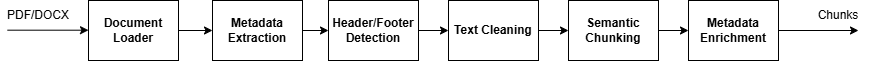
\includegraphics[width=\textwidth]{Figures/chunking_funes.png}
    \caption{Document chunking workflow implemented in the Storage Manager.}
    \label{fig:chunking_pipeline}
\end{figure}


\subsubsection{Embedding Generation}

After the document chunking phase, each generated text fragment is transformed into a numerical representation suitable for semantic retrieval. This process is performed by the embedding generation module, whose objective is to map textual information into a continuous vector space where semantically similar contents are represented by nearby vectors.

Similarly to the other components of the Storage Manager, the embedding generation layer was designed following an abstraction-based approach. The abstract class \texttt{EmbeddingModel} defines the interface required by the system, exposing a single operation responsible for converting a text input into its corresponding embedding vector.

This abstraction decouples the retrieval pipeline from the specific embedding model used during execution. Therefore, different embedding techniques can be integrated by implementing the same interface, without requiring modifications to the memory management or storage layers.

For the Proof of Concept, the selected implementation is based on the Sentence Transformer architecture through the \texttt{all-MiniLM-L6-v2} model. The model generates dense vector representations that capture semantic relationships between textual fragments, enabling similarity-based retrieval even when the query and the stored document use different wording.

The generated embeddings are computed during the document ingestion phase and stored together with the corresponding text chunks and metadata inside the vector database. During the retrieval phase, the same embedding model is used to encode the user query, allowing the system to perform semantic similarity comparison between the query representation and the indexed knowledge base.

The separation between embedding generation and storage management allows the system to remain independent from a specific embedding technology, facilitating future experimentation with alternative models or domain-specific embedding approaches.


\subsubsection{Vector Storage}

The vector storage layer is responsible for persisting document embeddings and supporting efficient similarity search operations. To preserve the modular architecture adopted throughout the Storage Manager, this functionality is defined through the abstract class \texttt{VectorStore}, which specifies the common interface required by the retrieval pipeline.

The interface exposes the basic operations required by any vector database implementation, including document insertion, similarity search, retrieval of the complete collection, and access to the content hashes used for duplicate detection. As a consequence, replacing the underlying vector database only requires implementing the same interface, while the higher-level components remain unchanged.

The Proof of Concept adopts ChromaDB as the concrete implementation through the \texttt{ChromaStore} class. This wrapper encapsulates all interactions with the database, including collection creation, persistent storage, document insertion, similarity search, and collection management.

During the ingestion phase, each chunk is stored together with its embedding vector and the corresponding metadata. The metadata are preserved inside the vector database and include information such as the document source, page number, chunk identifier, and content hash. This additional information is subsequently exploited during retrieval and traceability operations.

Before new chunks are inserted, the vector store exposes the set of already stored content hashes, allowing the Memory component to efficiently identify duplicate chunks and avoid redundant indexing.

During retrieval, the vector store performs similarity search by comparing the embedding of the user query with the embeddings stored in the collection, returning the most semantically relevant document fragments together with their associated metadata.


\subsubsection{Knowledge Memory Management}

The Memory component represents the central layer responsible for managing the lifecycle of the knowledge stored inside the Retrieval-Augmented Generation system. Its main purpose is to provide a unified interface for storing, updating, and retrieving information, while hiding the implementation details of the underlying storage and retrieval mechanisms.

Following the modular design adopted throughout the Storage Manager, the memory layer is defined through the abstract class \texttt{Memory}. This interface specifies the fundamental operations required by any memory implementation: adding new knowledge items, searching for relevant information, and retrieving the complete stored knowledge base.

This abstraction allows the retrieval pipeline to remain independent from the specific memory implementation. Different types of memories can therefore be introduced in the future, such as domain-specific knowledge bases or agent-specific memories, without requiring changes to the components responsible for document processing or storage.

The concrete implementation developed for the Proof of Concept is represented by the \texttt{KBMemory} class, which manages the knowledge base used by the multi-agent system. The class acts as an intermediate layer between the document processing components and the storage mechanisms, coordinating chunk generation, embedding computation, indexing, retrieval, and result refinement.

During the ingestion phase, the memory receives a document path and uses the configured chunker to transform the document into a collection of semantically meaningful chunks. Before inserting new information, the system performs a duplicate detection phase based on the content hash associated with each chunk. This mechanism prevents the same information from being stored multiple times, reducing redundancy and improving the efficiency of the retrieval process.

Only previously unseen chunks are processed further. Their embeddings are generated through the configured embedding model and stored together with the associated metadata inside the vector database. At the same time, the textual representation of each chunk is inserted into a lexical index based on BM25, enabling the system to combine semantic and keyword-based retrieval strategies.

The retrieval process is designed as a multi-stage pipeline rather than a simple similarity search. The first stage performs semantic retrieval using vector similarity, exploiting the contextual information captured by embeddings. In parallel, a lexical retrieval strategy based on BM25 identifies documents containing relevant keywords from the user query. 

For a requested retrieval size of \(k\), both the vector store and the BM25 index independently retrieve \(2k\) candidate chunks. The enlarged candidate set increases the probability of recovering relevant documents that may appear only in one of the two rankings before the fusion stage.

The results produced by the two retrieval mechanisms are then combined using the Reciprocal Rank Fusion (RRF) algorithm \cite{cormack2009reciprocal}. This approach allows the system to exploit the complementary strengths of both methods: vector retrieval improves semantic understanding, while lexical retrieval provides accurate matching for specific terms, identifiers, or technical expressions.


Given a document \(d\), its RRF score is computed as

\begin{equation}
RRF(d)=\sum_{r\in R}\frac{1}{k+\mathrm{rank}_r(d)}
\label{eq:rrf}
\end{equation}

where \(R\) denotes the set of ranked retrieval methods, \(\mathrm{rank}_r(d)\) is the rank assigned to document \(d\) by retrieval method \(r\), and \(k\) is a positive constant controlling the influence of lower-ranked documents. In the proposed implementation, the commonly adopted value \(k=60\) is used \cite{cormack2009reciprocal}.

Unlike score-based fusion methods, RRF does not require the normalization of similarity scores, which may originate from heterogeneous retrieval models and therefore be expressed on different scales. Instead, the fusion process relies solely on the relative ranking of retrieved documents, making the resulting ranking more robust and less sensitive to differences between lexical and semantic retrieval functions.

The fused ranking is finally refined through a Cross-Encoder reranker. While the initial retrieval stages evaluate query-document similarity independently, the Cross-Encoder jointly processes the query and each candidate chunk, allowing it to model deeper semantic interactions between the two texts.

This additional ranking stage is computationally more expensive than embedding-based retrieval and is therefore applied only to the limited set of candidate documents produced by the hybrid retrieval phase. The final ranked list returned by the reranker constitutes the contextual information provided to the upper layers of the multi-agent framework.

The resulting memory architecture therefore implements a complete retrieval pipeline composed of:

\begin{itemize}
    \item semantic retrieval through vector embeddings;
    \item lexical retrieval through BM25 indexing;
    \item rank fusion through Reciprocal Rank Fusion;
    \item relevance refinement through Cross-Encoder reranking.
\end{itemize}

This multi-stage approach improves the robustness of the knowledge retrieval process, reducing the limitations of relying on a single retrieval strategy and providing higher-quality contextual information to the decision-support agents.



\subsubsection{RAG Validation}

To evaluate the effectiveness of the implemented Retrieval-Augmented Generation pipeline, an experimental validation was conducted on a heterogeneous knowledge base composed of twenty technical documents. The dataset included both publicly available ECSS (European Cooperation for Space Standardization) standards and few internal technical documentation provided by Telespazio. The selected corpus reflects the type of documentation that the proposed decision support system is expected to process in real operational scenarios.

A benchmark composed of one hundred queries was manually created for the evaluation. Each query was manually formulated to capture the main semantic content of a randomly selected page while avoiding verbatim copying of the original text. For every query, the expected relevant page was manually annotated and considered as the ground truth.

The objective of the evaluation was to measure the capability of the retrieval pipeline to return the correct document among the retrieved candidates. Three retrieval configurations were evaluated:

\begin{itemize}
    \item semantic retrieval using only the vector database;
    \item hybrid retrieval using Reciprocal Rank Fusion (RRF);
    \item hybrid retrieval followed by Cross-Encoder reranking.
\end{itemize}

The performance was assessed using two standard Information Retrieval metrics:

\begin{itemize}
    \item \textbf{Recall@5}, measuring the percentage of queries for which the correct document appeared within the first five retrieved results;
    \item \textbf{Mean Reciprocal Rank (MRR)}, evaluating how early the correct document appeared in the ranking.
\end{itemize}

\begin{table}[H]
\centering
\caption{Retrieval performance obtained during the Storage Manager validation.}
\label{tab:rag_validation}
\begin{tabular}{lcc}
\toprule
Configuration & Recall@5 (\%) & MRR (\%)\\
\midrule
Vector Search & 79 & 68.48\\
Hybrid Search (RRF) & 86 & 71.78\\
Hybrid Search + Cross Encoder & \textbf{86} & \textbf{80.50}\\
\bottomrule
\end{tabular}
\end{table}


\begin{table}[H]
\centering
\caption{Position of the correct document within the retrieved Top-5 results.}
\label{tab:position_distribution}
\begin{tabular}{lccccc}
\toprule
Configuration & Rank1 & Rank2 & Rank3 & Rank4 & Rank5\\
\midrule
Vector Search & 61 & 11 & 4 & 1 & 2\\
Hybrid (RRF) & 62 & 14 & 4 & 5 & 1\\
Hybrid + Reranker & \textbf{76} & 7 & 3 & 0 & 0\\
\bottomrule
\end{tabular}
\end{table}

The obtained results highlight the contribution of each stage of the retrieval pipeline.

The introduction of hybrid retrieval through Reciprocal Rank Fusion increased the Recall@5 from 79\% to 86\%, demonstrating that combining semantic and lexical retrieval allows the system to recover relevant documents that may be overlooked by either retrieval strategy individually.

Although the increase in Mean Reciprocal Rank is more moderate (from 68.48\% to 71.78\%), the improvement indicates that the correct document is generally positioned closer to the top of the retrieved ranking.

The largest improvement is observed after introducing the Cross-Encoder reranker. While the Recall@5 remains unchanged, the MRR increases significantly from 71.78\% to 80.50\%. This behaviour is expected since the reranker does not retrieve additional documents but rather reorders the candidates already returned by the hybrid retrieval stage.

The position distribution further confirms this behaviour. The number of queries for which the correct document is ranked first increases from 62 to 76, while no relevant document appears in the fourth or fifth position after reranking. This demonstrates that the Cross-Encoder is particularly effective at improving the ranking quality of already retrieved candidates.